%% Page settings.
\documentclass[10pt,a4paper,twoside]{article}
\usepackage[top=1.2in, left=1.2in, bottom=1.2in, right=1.2in]{geometry}
%==================================================%
%% Encoding packages.
\usepackage[UKenglish]{babel}
\usepackage[nodayofweek]{datetime}
\usepackage[T1]{fontenc}
\usepackage[utf8]{inputenc}
\usepackage{amsmath}
\usepackage{amsthm}
\DeclareMathAlphabet\mathbb{U}{msb}{m}{n}
%\usepackage{amsfonts}
%\usepackage{amssymb}
\usepackage{calc}
\usepackage{natbib}
\usepackage{color}
\usepackage{subcaption}
%==================================================%
%% Document details.
\usepackage{titling}
\title{Information and admissible sets}
\author{Jeff Rowley}
\newcommand{\thedate}{\today}
% Enter document details here.
\newcommand{\details}{C:/Dropbox/TeXTemplates/}
% Enter the file path here for the UCL logo and bibliography.
% Change this file path for different computer systems.
\newcommand{\homePC}{C:/Users/Jeffro/Documents/}
\newcommand{\workPC}{U:/}
%==================================================%
%% Date macro.
\newcommand{\theseason}[1]{
\ifcase \month 
\or Winter\or Winter\or Spring\or Spring\or Spring\or Summer\or Summer\or Summer\or Autumn\or Autumn\or Autumn\or Winter\fi}
% Displays the season.
% Obsolete in this template.
%==================================================%
%% Useful packages.
\usepackage{enumerate}		% Lists.
\usepackage{bbm}			% Indicator functions.
\usepackage{lipsum}			% Random text generator.
\usepackage{MnSymbol}		% Arrows.
\usepackage{graphicx}		% Graphics.
%==================================================%
%% Theorem environments.
\newcounter{countthm}[section]
\newcounter{countlem}[section]
\newcounter{countex}[section]
% Creates new counters which reset at each new section. 
\renewcommand{\thecountthm}{\thesection.\arabic{countthm}}
\renewcommand{\thecountlem}{\thesection.\arabic{countlem}}
\renewcommand{\thecountex}{\thesection.\arabic{countex}}
% Redefines counters to include the section number.
\newtheorem{thm}[countthm]{Theorem}
% Creates a theorem environment - type \thm to begin.
\newtheorem{lem}[countlem]{Lemma}
% Creates a lemma environment - type \lem to begin.
\newtheorem{ex}[countex]{Example}
% Creates an example environment - type \ex to begin.
\newtheorem*{Acknowledgements}{Acknowledgements}
% Creates a thanks environment.
\newcommand{\newthm}[1]{\newtheorem*{#1}{#1}}
% A macro that makes defining new theorem environments quick.
% Type \newthm{<Theorem name here>} to begin.
%==================================================%
%% Math operators.
\DeclareMathOperator*{\plim}{plim}
% Writes plim in math environment - type \plim to enter.
\DeclareMathOperator*{\argmax}{argmax}
% Writes argmax in math environment - type \argmax to enter.
\DeclareMathOperator*{\argmin}{argmin}
% Writes argmin in math environment - type \argmin to enter.
\DeclareMathOperator*{\argsup}{argsup}
% Writes argsup in math environment - type \argsup to enter.
\DeclareMathOperator*{\arginf}{arginf}
% Writes arginf in math environment - type \arginf to enter.
\newcommand\independent{\protect\mathpalette{\protect\independenT}{\perp}} 
\def\independenT#1#2{\mathrel{\rlap{$#1#2$}\mkern2mu{#1#2}}} 
% Pastes an independence symbol - type \independent to enter.
\DeclareMathOperator*{\generates}{:.}
% Write generate symbol (identification).
\DeclareMathOperator*{\generated}{.:}
% Write generated symbol (identification).
%==================================================%
%% Abbreviations.
\newcommand{\US}{United States}
% Use \US macro when use is as a noun.
% Use U.S. when use is as an adjective.
%==================================================%
%% Equation numbering.
\numberwithin{equation}{subsection}
% Numbers equations up to the subsection. To change level,
% replace subsection with section.
%==================================================%
%% Counters.
\newcounter{saveenumi}
\newcounter{saveenumi1}
\setcounter{section}{0}
%==================================================%
\newcommand{\ESRC}{I acknowledge financial support from the Economic and Social Research Council (ESRC).}
%==================================================%
%% The title page.
\makeatletter				
% Changes @ to catcode 11.
\renewcommand{\@maketitle}{
\null
\graphicspath{ {\details} }
\flushleft{\includegraphics[width=40mm]{UCL_Logo_Orange}}
\hspace{5mm}
\normalsize Department of Economics, University College London\\
\vskip\bigskipamount
\leaders\vrule width \textwidth\vskip0.4pt 
\vskip\bigskipamount 
\nointerlineskip
% This completes the UCL banner.
\begin{center}
\begin{minipage}{100mm}
\begin{center}
\vspace{20mm}
\LARGE
\textbf{
\@title}
\par
\vspace{10mm}
\normalsize
\@author
\par
\vspace{5mm}
\normalsize
\thedate
\end{center}
\end{minipage}
\end{center}
}
\makeatother				
% Reverts @ to catcode 12.
%==================================================%
%% Packages to load at end of preamble. 
% Note conflict between Tkz-euclide package set and 
% game theory package set. Load one or the other.
\usepackage{hyperref}
%\usepackage[numbered]{mcode}

%% Tkz-euclide package set.
%\usepackage{tkz-euclide}
%\usepackage{pgfplots}
%\usepgfplotslibrary{external} 
%\tikzexternalize[prefix=tikz/]

%% Game theory package set.
\usepackage{pstricks}	
\usepackage{egameps}		 
\usepackage{pst-3d}			
\usepackage{sgame}	
\renewcommand{\gamestretch}{1.5}
%==================================================%
%% Further notes regarding egameps package.
% The egameps package is incompatible with this template
% due to UCL logo. Solution is to independently run 
% egameps through on a latex blank document, then insert 
% pdf into this document. Recall that to run egameps:
% "latex" --> "DVi->PS" --> "PS->PDF"
% then use "includegraphics[]" with trim option. 
%==================================================%
%% Headers and footers.
\usepackage{fancyhdr}
\pagestyle{fancy}
\renewcommand{\sectionmark}[1]{\markright{\thesection.\ #1}}
% This redefines the \rightmark command so that the section number does not appear.
% NOTE: To remove the section number, delete <<\thesection.\>>
\lhead[\thepage]{\rightmark}
\rhead[\rightmark]{\thepage}
\chead[]{}
\cfoot[]{}
%\lfoot[\thetitle]{}
%\rfoot[]{\theauthor}
\renewcommand*\thesection{\arabic{section}}
\usepackage{epigraph}
%==================================================%
%% Start of document.
\begin{document}
\maketitle
\vspace{10mm}
\begin{abstract}
\noindent <<Abstract here>>
\begin{Acknowledgements}
<<Acknowledgements here>>
\ESRC
\end{Acknowledgements}
\end{abstract}
\vspace{5mm}
%==================================================%
%% Document.
%==================================================%
I explore the effect of incorporating information for a non-parametric binary choice model. The model permits endogenous variation in a scalar random variable due to non-random selection, and it is the average causal effect of this endogenous variable on the outcome variable that is of interest. The model embeds an exclusion restriction and an independence restriction that together define an instrumental variable but is silent as to the relationship between the endogenous variable and the instrumental variable. I restrict the relationship between the outcome variable and the endogenous variable up to a non-parametric threshold crossing function. The model is credible \citep{book.manski} in that it embeds only weak non-verifiable restrictions, but does not identify the average causal effect of the endogenous variable on the outcome variable.\footnote{Assumptions that cannot be tested using data; the model does embed some non-trivial non-verifiable restrictions that might be relaxed.} Rather, the model partially identifies the average causal effect of the endogenous variable on the outcome variable. 

I define information to be those additional characteristics of economic agents that are observable with the caveat that these characteristics be exogenous and relevant to the latent structure. It is convenient to think of such characteristics as being predetermined and immutable; characteristics that result from choices that are made jointly with the outcome variable are excluded by the definition. Accordingly, exogenous variables and instrumental variables are each regarded as information, and I distinguish between these classes of information. I study how the admissible set of values for the average causal effect of the endogenous variable on the outcome variable changes as each class of information is incorporated into the model separately. 

It is useful to distinguish between classes of information since each class enters the latent structure in a different way. Exogenous variables are permitted to enter the structural equation for the outcome variable and to determine the endogenous variable. As such, exogenous variables can be seen to enrich both individual response and individual selection, respectively. An important consequence is that the causal effect of the endogenous variable on the outcome variable depends upon the value of the exogenous variables when individual response is enriched. In contrast, instrumental variables are excluded from the structural equation for the outcome variable by definition and so only enrich individual selection. Given this, the effect of incorporating information is different depending upon the class of information that is being incorporated into the model.  

Incorporating information of any class is generally sensible for a number of reasons. Firstly, incorporating information is known to be efficient; variation that is attributable to an observable variable is instead attributable to unobservable heterogeneity when that variable is omitted. Secondly, the effect of incorporating information for partially identifying models is not well-documented; one hypothesis is that incorporating information narrows bounds on admissible sets. Such an effect is not documented in identifying models precisely because such models deliver a point estimate (a set of length zero), but point estimates may shift as information is incorporated. A contribution that I make is in showing that \color{red} incorporating information leads to narrower bounds on the admissible sets \color{black} that are delivered by the aforementioned model. A further reason to particularly favour incorporating exogenous variables is that the average causal effect of the endogenous variable on the outcome variable in identifiable sub-populations can be recovered. I name this structural characteristic the conditional average causal effect of the endogenous variable on the outcome variable, and index it by the conditioning value.\footnote{The conditioning value is specifically the value of the exogenous variables. \cite{hEvY05} defines a parameter $ATE(x)$ that is equivalent to the conditional average causal effect of the endogenous variable on the outcome variable at the conditioning value $x$. \cite{kHt10} and \cite{13.misc.abrevaya} instead refer to this parameter as the conditional average treatment effect and abbreviate this as $CATE(x)$.} Understanding the effect of an intervention in sub-populations can be interesting if the intervention can be targeted or if the intervention is to be applied elsewhere in a population that differs according to its observable characteristics. 




%I define information to be those additional characteristics of economic agents that are observable with the caveat that these characteristics be exogenous and relevant to the latent structure. It is convenient to think of such characteristics as being predetermined and immutable; characteristics that result from choices that are made jointly with the outcome variable are excluded by the definition. Accordingly, exogenous variables and instrumental variables are regarded as information. I study how the admissible set of values for the average causal effect of the endogenous variable on the outcome variable changes as each class of information is incorporated separately.
%
%It is useful to distinguish between different classes of information since each class enters the latent structure in a different way. Exogenous variables enter the structural equation for the outcome variable and so can be seen to enrich individual response. A consequence is that the average causal effect of the endogenous variable on the outcome variable is conditional upon the value that the exogenous variables are held fixed at. This conditionality is noted in \cite{hEvY05}. I name this structural characteristic the conditional average causal effect of the endogenous variable on the outcome variable and index it by the conditioning value.\footnote{\cite{hEvY05} defines a parameter $ATE(x)$ that is equivalent to the average causal effect of the endogenous variable on the outcome variable. \cite{kHt10} and \cite{13.misc.abrevaya} instead refer to this parameter as the conditional average treatment effect and abbreviate this as $CATE(x)$.} Instrumental variables do not enter the structural equation for the outcome variable and so only enrich individual selection.  
%
%Incorporating information is generally sensible for a number of reasons. Firstly, understanding the effect of an intervention in various sub-populations can be interesting. This is particularly true if the intervention can be targeted, or if the intervention is to be applied elsewhere in a population that differs according to its observable characteristics. Conditional average causal effects develop a more detailed picture of the distribution of the effect of an intervention. Secondly, incorporating information is known to be efficient; variation that is attributable to an observable variable is instead attributed to unobservable heterogeneity when that variable is omitted. Thirdly, the effect of incorporating information for partially identifying models is not well-documented; one hypothesis is that incorporating information leads to narrower bounds on admissible sets. Such an effect is not documented in identifying models precisely because such models deliver a point estimate (a set of length zero), but point estimates may shift as information is incorporated. A contribution that I make is in showing that \color{red} incorporating information leads to narrower bounds on the admissible sets \color{black} that are delivered by the aforementioned model. 
%
%The non-parametric binary choice model that I assume is the same as that in \cite{cr13} except that I enrich individual behaviour. The distinction is that \cite{cr13} allow only the endogenous variable to determine the threshold 
%
%
%

%A complication of working with partially identifying models is in determining the admissible set of values for a structural characteristic of interest. Fortunately, application of random set theory to economics  

%Determining the admissible set of values for the average causal effect of the endogenous variable on the outcome variable and establishing that the bounds on this set are sharp has been made easier by the application of random set theory to economics. 
%
%
%
%
%This paper is an extension of \cite{cr13}. Like \cite{cr13}, I specify a non-parametric model that embeds a threshold crossing restriction and study the admissible set of values for the average causal effect of the endogenous variable on the outcome variable that is delivered by this model. \cite{cr13} estimates the admissible set of values for the average causal effect of the endogenous variable on the outcome variable and compares this to estimates of the local average treatment effect.\footnote{It should be noted that these are not only distinct parameters but that each is identified (or partially identified) under a non-nested set of restrictions.} In contrast, my interest is only in the average causal effect of the endogenous variable on the outcome variable. As in \cite{cr13}, estimates are for data on female labour force participation in the \US , but I also derive general conditions on the probability distribution of observable variables that are necessary for each model to deliver different bounds. 


%==================================================%
\section*{Notation}
There is a probability space $(\Omega,\Sigma,\mathbb{P})$ on which are defined random variables $(Y,D,X,Z,U)$. Here, $(Y,D,X,Z)$ are observable with supports $(\mathcal{R}_Y,\mathcal{R}_D,\mathcal{R}_X,\mathcal{R}_Z)$, and $U$ is unobservable with as yet unspecified support. I allow $(X,Z,U)$ to be vectors, in which case the support is given by the Cartesian product of the supports of each element in the vector. I refer to $Y$ as the outcome variable, to $D$ as the endogenous variable, to $X$ as the exogenous variable, to $Z$ as the instrumental variable, and to $U$ as unobservable heterogeneity. The logic of this naming convention will be made clear by the restrictions that are imposed upon these random variables in the main text. Lower case letters are used to represent specific values of these random variables.

I denote by $Y(d)$ the counterfactual value of $Y$ when $D$ is externally fixed, and by $D(z)$ the counterfactual value of $D$ when $Z$ is externally fixed. I denote by $\mathbb{E}$ the expectation operator, and  by $\mathbbm{1}$ the indicator function. Related to these concepts are the average causal effects $ACE(D\rightarrow Y)$ and $ACE(Z\rightarrow D)$ that are defined as $\mathbb{E}[Y(d_1)-Y(d_0)]$ and $\mathbb{E}[D(z_1)-D(z_0)]$ that are well-defined when $D$ and $Z$ are binary, respectively. To distinguish between population and sample quantities, I subscript sample quantities by $n$. 

Further terminology and notation is introduced in Figure~\ref{fig:models} through Figure~\ref{fig:partials}. This specifically relates to models and structures, and is consistent with the approach that is formally laid out in \cite{h50} and in \cite{krE50}. Following \cite{h50} I also adopt the notation $S\generates P$ that signifies that a structure $S$ generates a probability distribution (of observable variables) $P$, and $P\generated G$ that signifies that $P$ is generated by $S$. 
%==================================================%
\section{A threshold crossing model}

%==================================================%
%% Diagrams
%==================================================%
\begin{figure}[p]
\centering
\begin{subfigure}{0.8\textwidth}
  \centering
  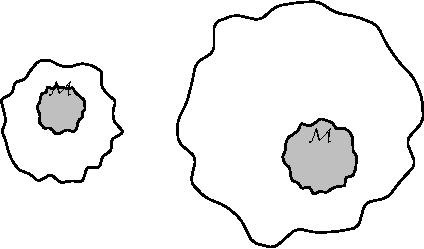
\includegraphics[width=\textwidth]{U:/GitHub/Covariatesets/Diagrams/Identification.pdf}
  \caption{A model $\mathcal{M}$ is a set of structures that forms a proper subset of the class of all structures $\mathcal{S}$. Each structure in $\mathcal{M}$ generates a probability distribution in the class of all probability distributions (of observable variables) $\mathcal{P}$. Then the image $\mathcal{I}$ is the set of all probability distributions that are generated by structures in $\mathcal{M}$.}
  \label{fig:model}
  \end{subfigure}
\begin{subfigure}{0.8\textwidth}
  \centering
  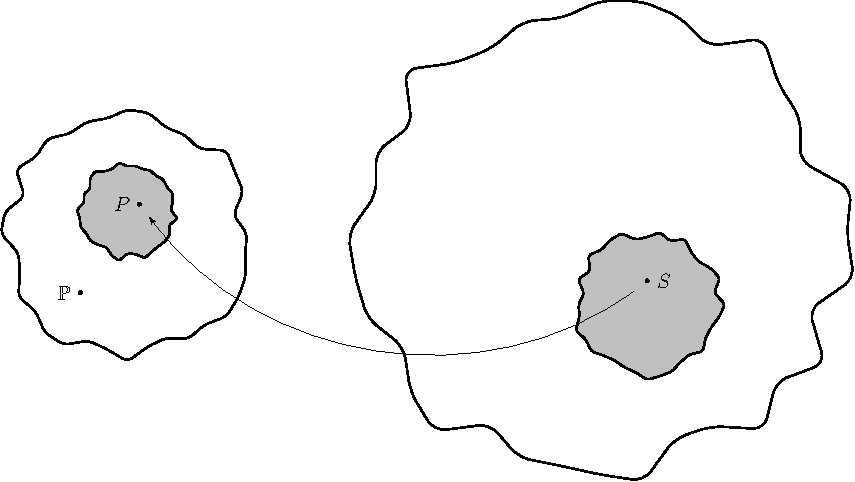
\includegraphics[width=\textwidth]{U:/GitHub/Covariatesets/Diagrams/Observationalrestrictiveness.pdf}
  \caption{A structure $S$ is incompatible with data if it generates a probability distribution (of observable variables) $P$ that is distinct from a realised probability distribution $\mathbb{P}$. If all structures in $\mathcal{M}$ are incompatible with data then $\mathcal{M}$ is said to be observationally restrictive, and is falsified. This condition is equivalent to $\mathbb{P}\in\mathcal{P}\setminus\mathcal{I}$.}
  \label{fig:obs.restrict}
  \end{subfigure}
\caption{Structures, models, probability distributions (of observable variables), and falsifiability.}
\label{fig:models}
\end{figure}
%==================================================%
\begin{figure}[p]
\centering
\begin{subfigure}{0.8\textwidth}
  \centering
  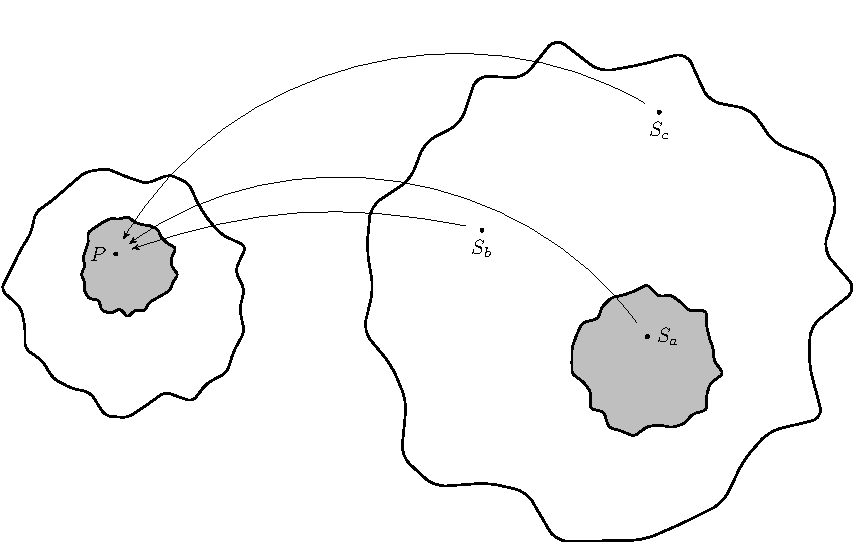
\includegraphics[width=\textwidth]{U:/GitHub/Covariatesets/Diagrams/Pointidentification.pdf}
  \caption{A model $\mathcal{M}$ is said to identify a structure $S$ if the probability distribution (of observable variables) $P$ that is generated by $S$ is distinct from those generated by other structures in $\mathcal{M}$. The structures $S_a$, $S_b$ and $S_c$ are said to be observationally equivalent as they all generate $P$ but $S_b$ and $S_c$ are not admitted by $\mathcal{M}$. As $S_a$ is the only structure that is admitted by $\mathcal{M}$ and that generates $P$, $S_a$ is identified by $\mathcal{M}$. For completeness, $\mathcal{M}$ is said to be uniformly identifying if it identifies each structure that it admits.}
  \label{fig:identify}
  \end{subfigure}
  \begin{subfigure}{0.8\textwidth}
  \centering
  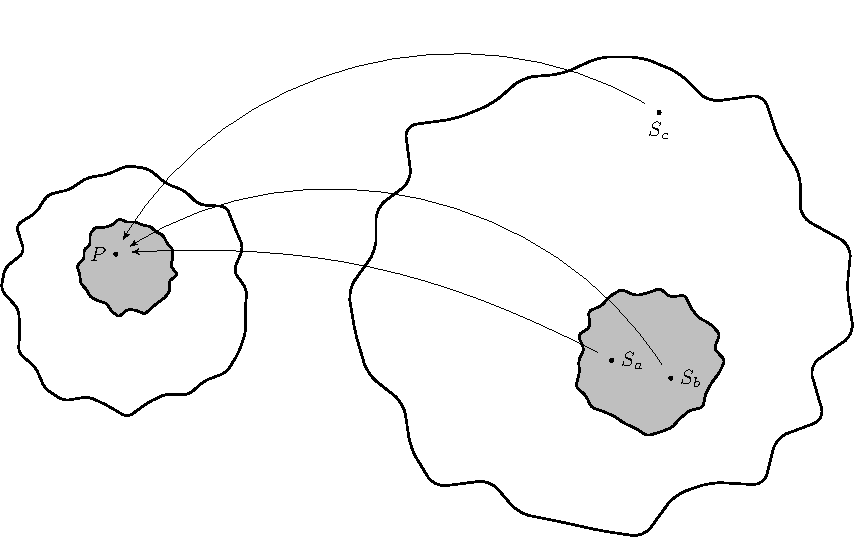
\includegraphics[width=\textwidth]{U:/GitHub/Covariatesets/Diagrams/Setidentification.pdf}
  \caption{As $S_a$ and $S_b$ are observationally equivalent and are both admitted by $\mathcal{M}$ then $\mathcal{M}$ does not identify either $S_a$ or $S_b$. Nonetheless, as $\mathcal{M}$ restricts the set of observationally equivalent structures that generate $P$ to $S_a$ and $S_b$ then $\mathcal{M}$ partially identifies $S_a$ (and $S_b$ to within $\lbrace S_a,S_b\rbrace$).}
  \label{fig:partial}
  \end{subfigure}
\caption{Identification and non-identification of a structure, and partial identification of a structure.}
\label{fig:identification}
\end{figure}
%==================================================%
\begin{figure}[p]
\centering
\begin{subfigure}{0.8\textwidth}
  \centering
  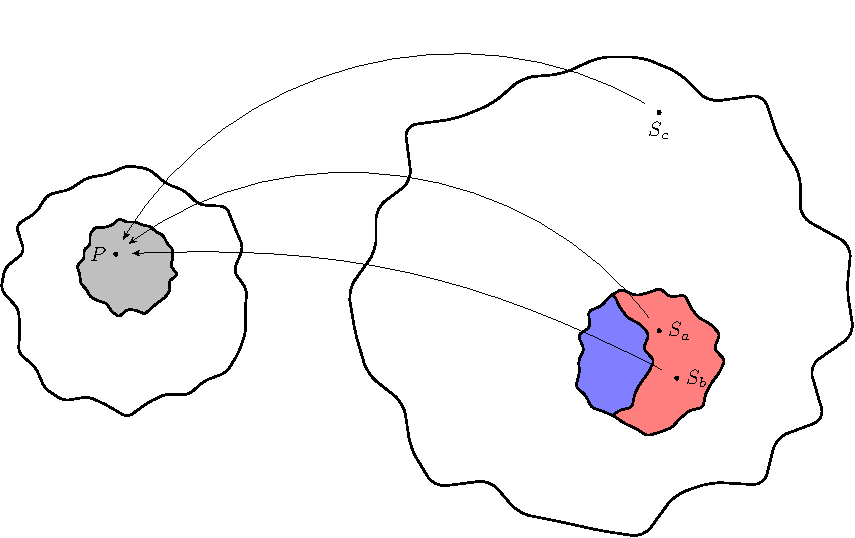
\includegraphics[width=\textwidth]{U:/GitHub/Covariatesets/Diagrams/Characteristic.pdf}
  \caption{A structural characteristic $\chi$ is a function of a structure $S$. A model $\mathcal{M}$ can be partitioned such that structures in a partition deliver the same value for $\chi$. Structures in the red partition $\color{red}\mathcal{M}$ deliver the value $a$ for $\chi$, and structures in the red partition $\color{blue}\mathcal{M}$ deliver the value $b$ for $\chi$. If $\chi$ is constant across all observationally equivalent structures that $\mathcal{M}$ admits then $\mathcal{M}$ is said to identify $\chi$. As $\chi(S_a)$ is equal to $\chi(S_b)$ (is equal to $a$) $\mathcal{M}$ identifies $\chi$.}
  \label{fig:characteristic}
  \end{subfigure}
  \begin{subfigure}{0.8\textwidth}
  \centering
  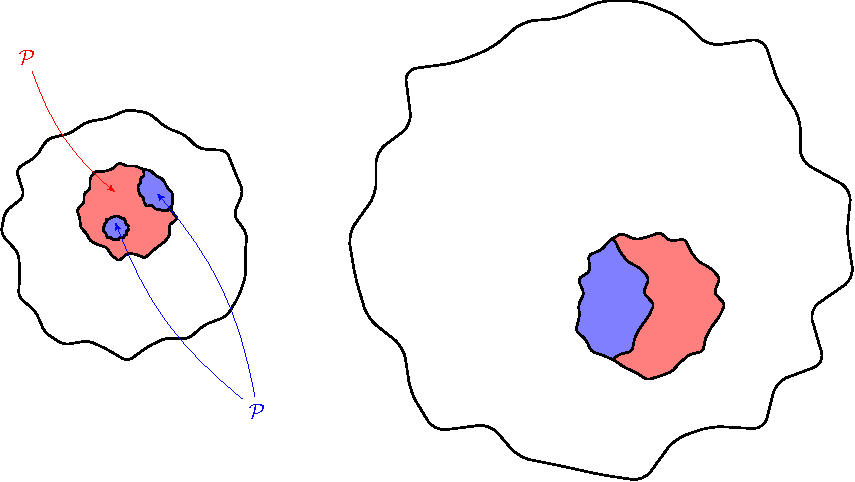
\includegraphics[width=\textwidth]{U:/GitHub/Covariatesets/Diagrams/Uniform.pdf}
  \caption{If $\mathcal{M}$ identifies $\chi$ for all structures in $\mathcal{M}$ then $\mathcal{M}$ is said to uniformly identify $\chi$. The class of all probability distributions (of observable variables) is partitioned into the blue partition $\color{red}\mathcal{P}$ and into the red partition $\color{blue}\mathcal{P}$. Probability distributions in $\color{red}\mathcal{P}$ are generated by (potentially many) structures in $\color{red}\mathcal{M}$, and probability distributions in $\color{blue}\mathcal{P}$ are generated by (potentially many) structures in $\color{blue}\mathcal{M}$. It is important that the number of partitions in $\mathcal{M}$ and in $\mathcal{P}$ are equal, although that number can be countably infinite. In the context of Figure~\ref{fig:uniform} $\mathcal{M}$ uniformly identifies $\chi$ since observationally equivalent structures that $\mathcal{M}$ admits are in the same colour of $\mathcal{M}$. More conveniently, whether $\mathcal{M}$ uniformly identifies $\chi$ can be determined by the existence of an identifying correspondence $G$, a functional. $\color{red}P$ is a probability distribution in $\color{red}\mathcal{P}$, and $\color{blue}P$ is a probability distribution in $\color{blue}\mathcal{P}$. Then $\mathcal{M}$ uniformly identifies $\chi$ if the value of $G(\color{red}P\color{black})$ is $a$ and if the value of $G(\color{blue}P\color{black})$ is $b$, holding for any such $\color{red}P$ and $\color{blue}P$. Notice that if $\mathcal{M}$ uniformly identifies all $\chi$ then $\mathcal{M}$ also uniformly identifies structures.}
  \label{fig:uniform}
  \end{subfigure}
  \caption{The identification of structural characteristics, and identifying correspondences.}
  \label{fig:characteristics}
\end{figure}
%==================================================%
\begin{figure}[p]
\centering
\begin{subfigure}{0.8\textwidth}
\centering
\caption{A structural characteristic $\chi$ is a function of a structure $S$. A model $\mathcal{M}$ can be partitioned such that structures in a partition deliver the same value for $\chi$. Structures in the red partition $\color{red}\mathcal{M}$ deliver the value $a$ for $\chi$, structures in the blue partition $\color{blue}\mathcal{M}$ deliver the value $b$ for $\chi$, and structures in the yellow partition $\color{yellow}\mathcal{M}$ deliver the value $c$ for $\chi$. The class of all probability distributions (of observable variables) $\mathcal{P}$ is partitioned into the red partition $\color{red}\mathcal{P}$, into the blue partition $\color{blue}\mathcal{P}$, into the yellow partition $\color{yellow}\mathcal{P}$ and into the grey partition $\color{gray}\mathcal{P}$. Probability distributions in a colour of $\mathcal{P}$ are generated by (potentially many) structures in the same colour of $\mathcal{M}$; the exception is probability distributions in $\color{gray}\mathcal{P}$ which are generated by (potentially many) structures in $\color{red}\mathcal{M}$ and in $\color{yellow}\mathcal{M}$. $P$ is a probability distribution in $\mathcal{P}$ with probability distributions defined similarly for each colour in $\mathcal{P}$.}
\end{subfigure}
\begin{subfigure}{0.8\textwidth}
  \centering
  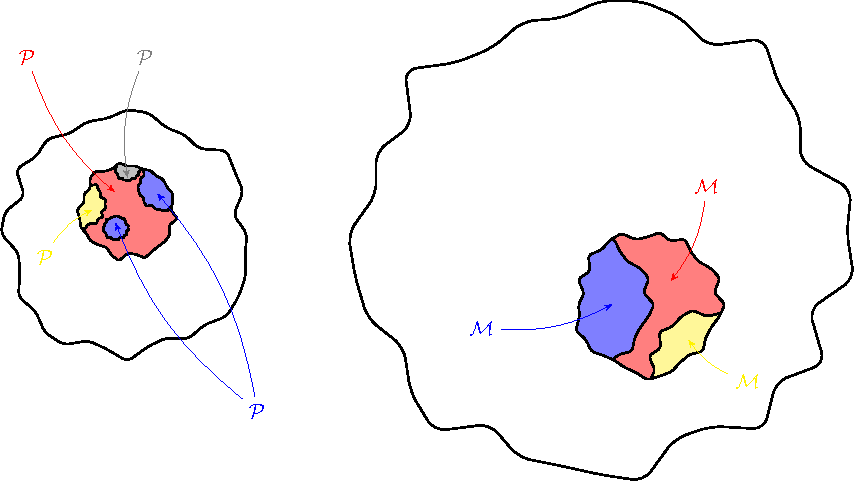
\includegraphics[width=\textwidth]{U:/GitHub/Covariatesets/Diagrams/Partial.pdf}
  \caption{That probability distributions in $\color{gray}\mathcal{P}$ are generated by structures in $\color{red}\mathcal{M}$ and in $\color{yellow}\mathcal{M}$ creates a complication; the value of $\chi$ is not constant across observationally equivalent structures that $\mathcal{M}$ admits and that generate a probability distribution in $\color{gray}\mathcal{P}$. So $\mathcal{M}$ does not uniformly identify $\chi$. Consideration of the identifying correspondence $G$ determines that this corresponds to there being structures in $\mathcal{M}$ for which $G$ does not deliver the value of $\chi$ when applied to the probability distributions that these structures generate. Nonetheless, if $\mathcal{M}$ restricts the set of values of $\chi$ for any probability distribution in $\mathcal{P}$ then $\mathcal{M}$ does have some non-trivial identifying power for $\chi$. Then $\mathcal{M}$ is said to uniformly partially identify $\chi$ if $\mathcal{M}$ and $\mathcal{P}$ can each be partitioned into countably many disjoint subsets and that a probability distribution in a partition of $\mathcal{P}$ is not generated by a structure in at least one partition of $\mathcal{M}$, holding for any such partition of $\mathcal{P}$. In the context of Figure~\ref{fig:partials} $\color{red}\mathcal{M}$ identifies $\chi$ up to $\lbrace a,c\rbrace$, $\color{blue}\mathcal{M}$ identifies $\chi$ uniquely to $b$, and $\color{yellow}\mathcal{M}$ identifies $\chi$ up to $\lbrace a,c\rbrace$. Each partition of $\mathcal{P}$ includes probability distributions that are generated by structures in at least one partition of $\mathcal{M}$. Equivalently, if $G$ is permitted to be a multivalued functional (or one-to-many) then $\mathcal{M}$ uniformly partially identifies $\chi$ if $G$ exists and if $G(P)$ contains the set of values of $\chi$ that are delivered by structures that generate $P$, holding for all such $P$. A caveat must be applied here; $G$ cannot be trivial in the sense that it is constant across all such $P$. Clearly this definition of $G$ does not exclude the possibility that there is multiplicity of identifying correspondences that satisfy this property. Sharpness is a desirable property in such circumstances; a functional $G$ that can be shown to deliver smaller sets according to some well-defined distance measure across all possible $P$ (and that satisfies the properties above) should be preferred to any alternative identifying correspondence.}
  \label{fig:partial1}
  \end{subfigure}
  \caption{Partial identification of a structural characteristic.}
  \label{fig:partials}
\end{figure}
%==================================================%
%% Bibliography.
\bibliographystyle{chicago}
\bibliography{\details Bibliography}
\end{document}

%I explore the effect of incorporating information on the identified set of values for the average causal effect of an endogenous variable on an outcome variable (the parameter of interest) that is delivered by a non-parametric model that embeds an exclusion restriction and an independence restriction that together characterise an instrumental variable. Endogenous variation enters the model since agents are permitted to non-randomly select a scalar observable characteristic. I consider the effect of combining many instrumental variables into a composite instrumental variable with many points of support on the identified set of values for counterfactual outcome distributions. Further, I consider the effect of enriching individual behaviour by allowing relevant exogenous variables to affect individual choice; specifically, I allow these variables to enter the structural equations that determine the endogenous variable and that determine the outcome variable. I establish the conditions under which the parameter of interest in the enriched model is equivalent to the parameter of interest in a model that does not explicitly account for the contribution of additional relevant exogenous variables. 
%
%The model that I consider partially identifies the parameter of interest. That is, the restrictions on the set of admissible structures (or data generating processes) that are implied by the model are insufficient to exclude observationally equivalent structures that deliver different values of the parameter of interest. The restrictions that are implied are nonetheless sufficient to restrict the set of values of the parameter of interest up to a non-trivial set. This concept is described graphically in Figure~\ref{fig:partials}. 
%\section{A}
%The model that I consider is partially identifying. That is, the restrictions on the set of admissible structures (or data generating processes) that are implied by the model are insufficient to exclude observationally equivalent structures. Furthermore, the model is unable to identify the structural characteristic of interest 
%
%\section{B}
%I explore the effect of incorporating information on the identified set of values for the average causal effect of an endogenous variable on an outcome variable (the parameter of interest) that is delivered by a non-parametric model. The model is weakly restrictive in that it does not embed a structural equation 
%
%
% that embeds an exclusion restriction and an independence restriction that together characterise an instrumental variable. The model is weakly restrictive in that it 
% 
%\section{C}
%Points to make:
%\begin{itemize}
%\item Non-parametric IV model with endogenous variable
%\item Non-random selection
%\item Average causal effect of endogenous variable on outcome variable is parameter of interest
%\item Model partially identifies the parameter of interest
%\item Model is weakly restrictive in that it does not specify a distribution for unobserved heterogeneity (imposes a normalisation and allows all distributional assumption to enter the non-parametric threshold function) and does not specify a selection equation
%\item Credible identification
%\item Want to incorporate additional information for the purpose of efficiency and to potentially provide tighter bounds on parameter of interest; may also be that conditional parameter of interest is useful
%\end{itemize}
%Related literature:
%\begin{itemize}
%\item \cite{cr13} The starting point for analysis
%\item \cite{crs13} Characterise level sets and identification
%\item \cite{bp97} Binary treatment characterise the identified set under non-compliance; weaker restrictions than presented here
%\item \cite{kI09} Continuous outcome variable; nesting of identified set under different model assumptions
%\item \cite{bLpO03} Average structural function when continuous endogenous regressor
%\item \cite{bEmOImOF12} Random set theory
%\end{itemize}